\chapter{Numerical Experiments}
\label{ch:numeric}

The ESI methods described in Chapter \ref{ch:review} are tested using synthetic data and evaluated using the metrics defined in the same chapter.

The synthetic data was created using anatomical data from the ICBM 152 template[]. 
%
As the name suggests, the ICBM152 template was constructed as an `average' of T1 MRI scans from 152 subjects.

Segmentation and surface extraction were omitted since these surfaces are provided with the template, and the methods for segmentation and surface extraction are not the focus of this work.
%
Those triangulated surfaces are displayed in figure \ref{fig:surfaces}.

\begin{figure}
\centering
%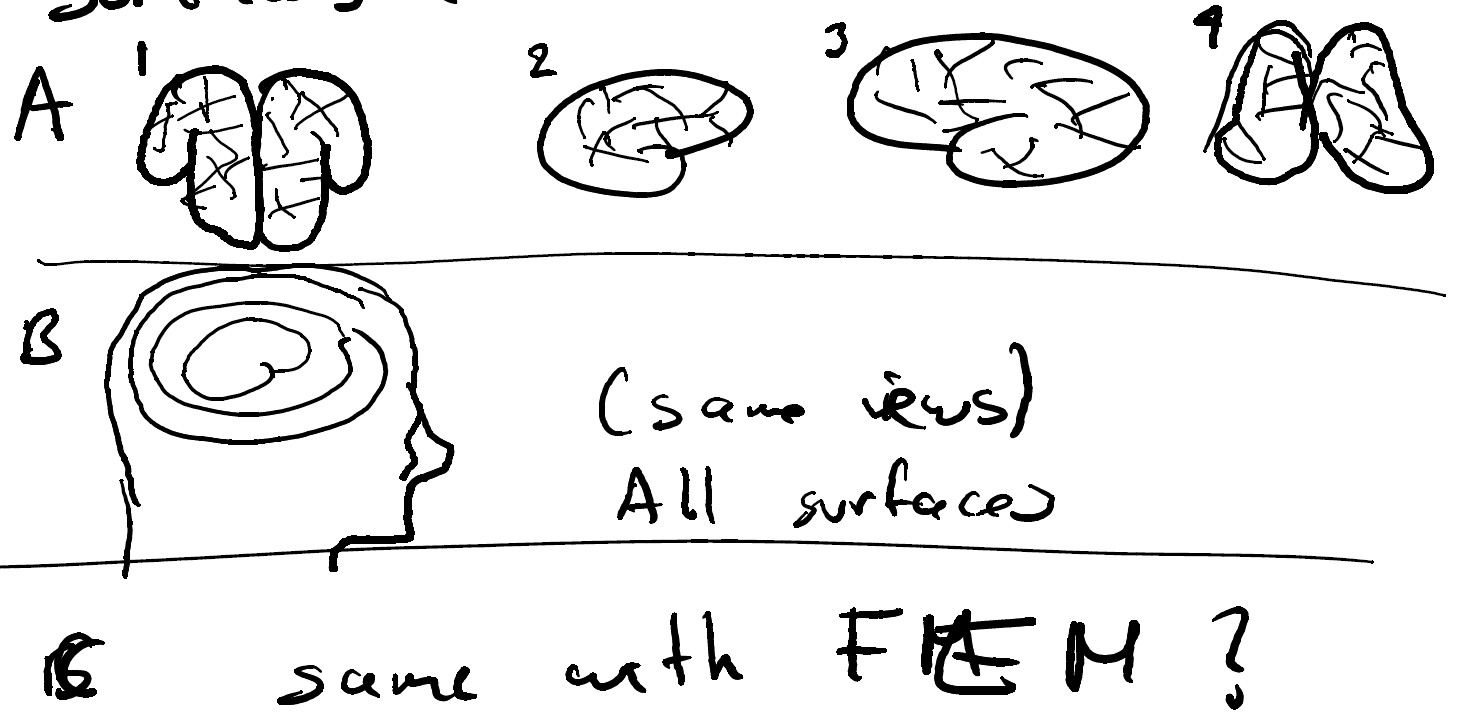
\includegraphics[width=0.8\linewidth]{./img_dev/nsSetupForward}
%
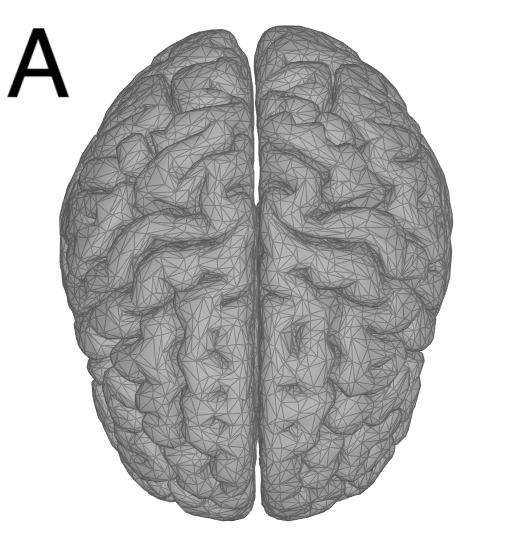
\includegraphics[width=0.18\linewidth]{./img_dev/3D_Subject_ICBM152_2019b_top - Copy2}
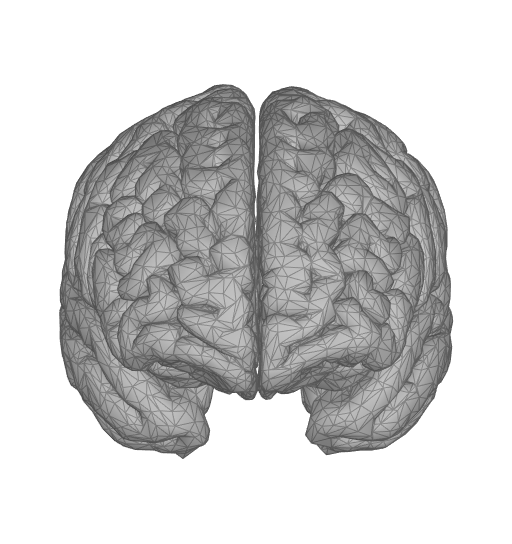
\includegraphics[width=0.18\linewidth]{./img_dev/3D_Subject_ICBM152_2019b_front}
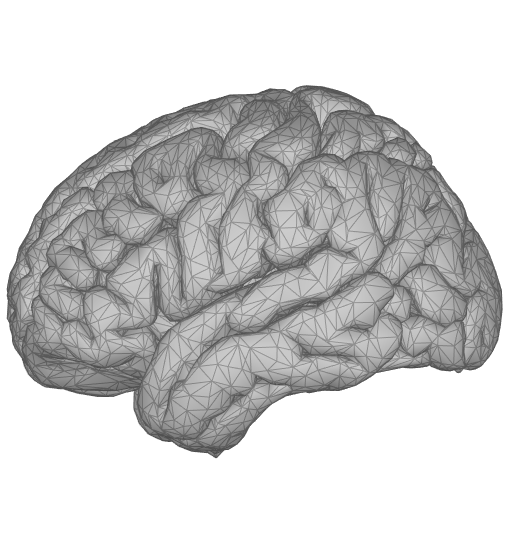
\includegraphics[width=0.18\linewidth]{./img_dev/3D_Subject_ICBM152_2019b_left}
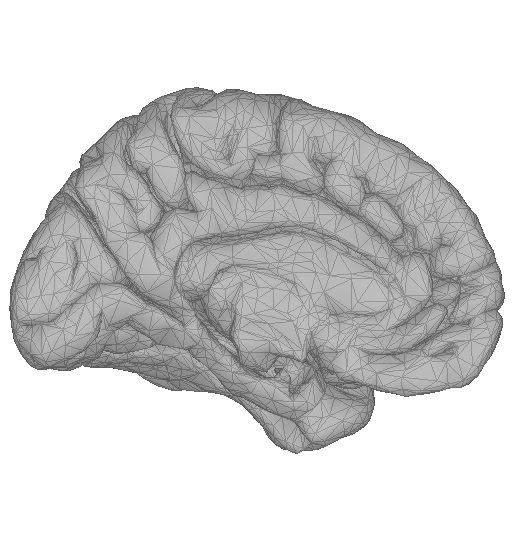
\includegraphics[width=0.18\linewidth]{./img_dev/3D_Subject_ICBM152_2019b_left_inner}
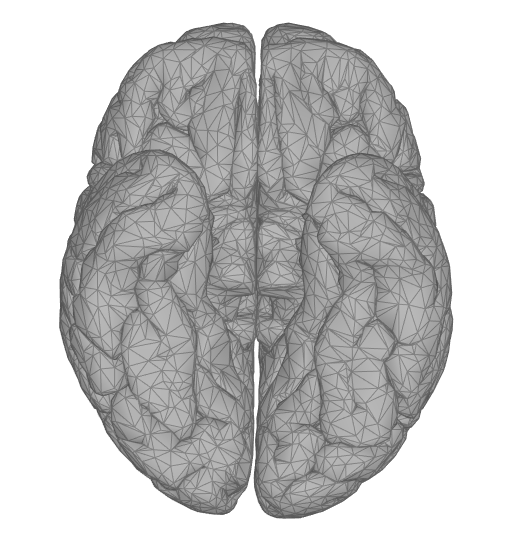
\includegraphics[width=0.18\linewidth]{./img_dev/3D_Subject_ICBM152_2019b_bottom}
%
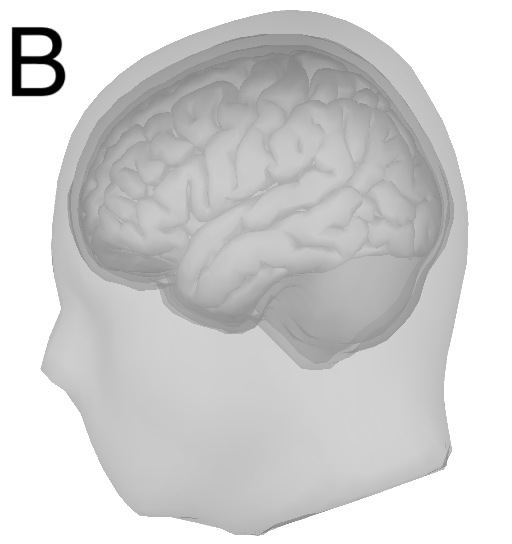
\includegraphics[width=0.2\linewidth]{./img_dev/combined - Copy}
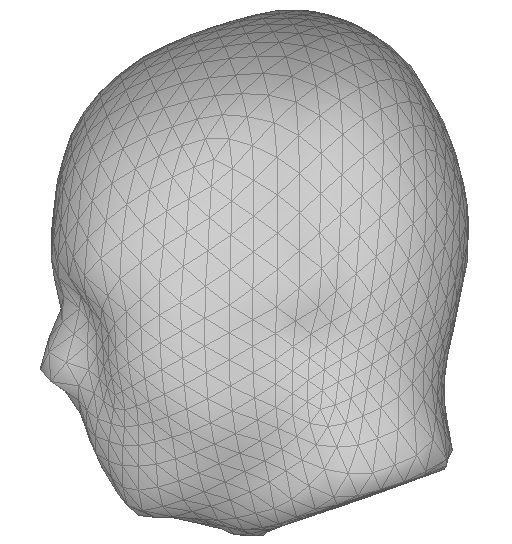
\includegraphics[width=0.18\linewidth]{./img_dev/combined_scalp}
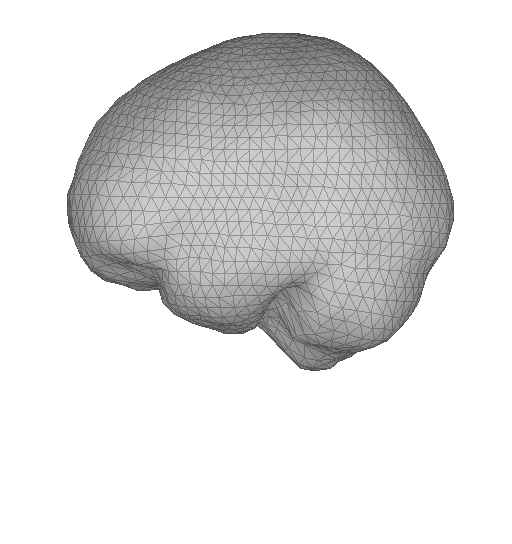
\includegraphics[width=0.18\linewidth]{./img_dev/combined_skull_outer}
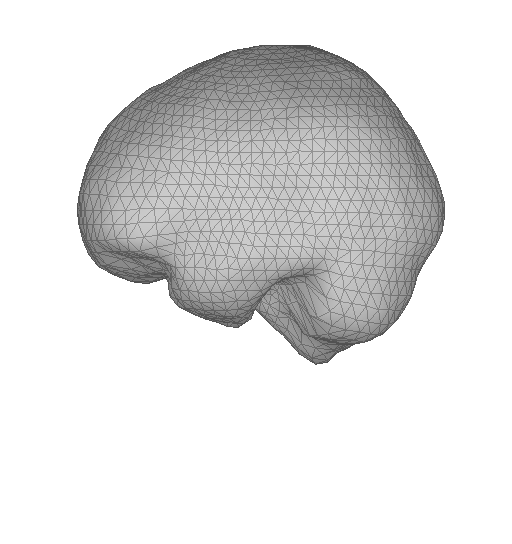
\includegraphics[width=0.18\linewidth]{./img_dev/combined_skull_inner}
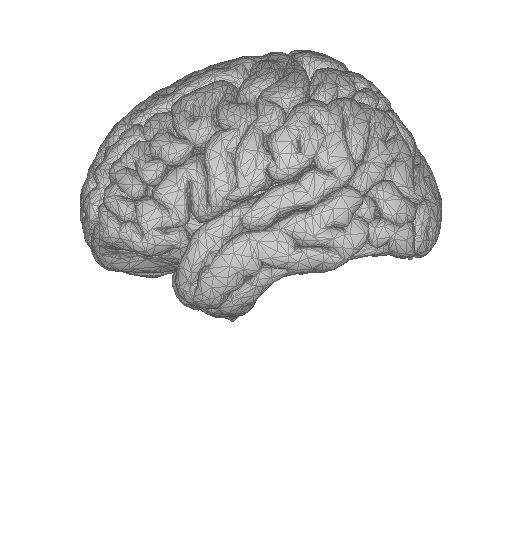
\includegraphics[width=0.18\linewidth]{./img_dev/combined_cortex}
\caption{A. Cortex surface for the ICBM 152 template, consisting of 15,002 vertices. Views from top, left, right, back. B. Triangulated surfaces used for the 4-sphere forward model: cortex, inner skull, outer skull, head.}
\label{fig:surfaces}
\end{figure}

Electrodes were placed according to the 10-10 International System [], resulting in $M=90$ electrodes. See either figure \ref{fig:1010system} for visual reference or [] for a more precise description of the electrode placement protocol.
%
The electrodes would be re-referenced to the average, so no reference electrode is considered at this stage.

Dipole locations were determined using the $N=15,002$ available in the triangulated cortex surface.
%
Dipole orientations were assumed to be orthogonal to the cortex surface.

Additionally, this section considers only a single time stamp, $ T=1$, for illustrative purposes.

\begin{figure}
\centering
%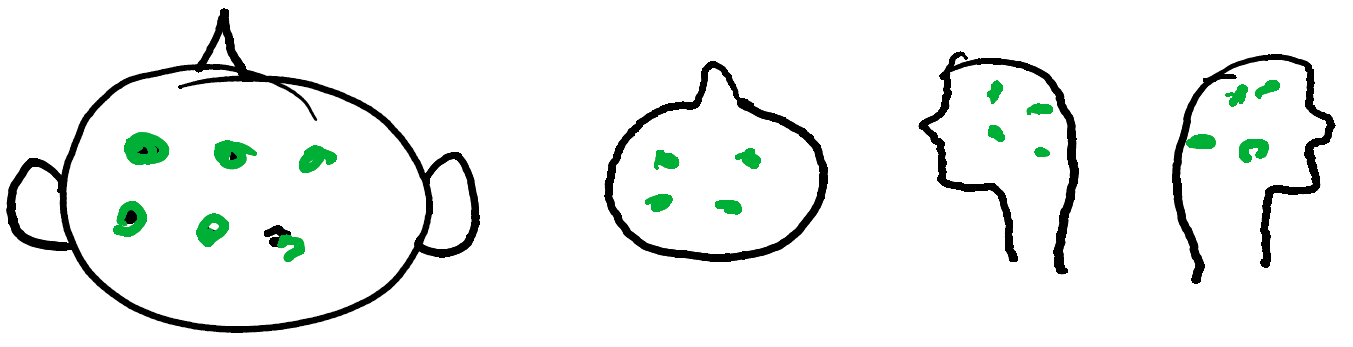
\includegraphics[width=0.8\linewidth]{./img_dev/nsElectrodeSetup}
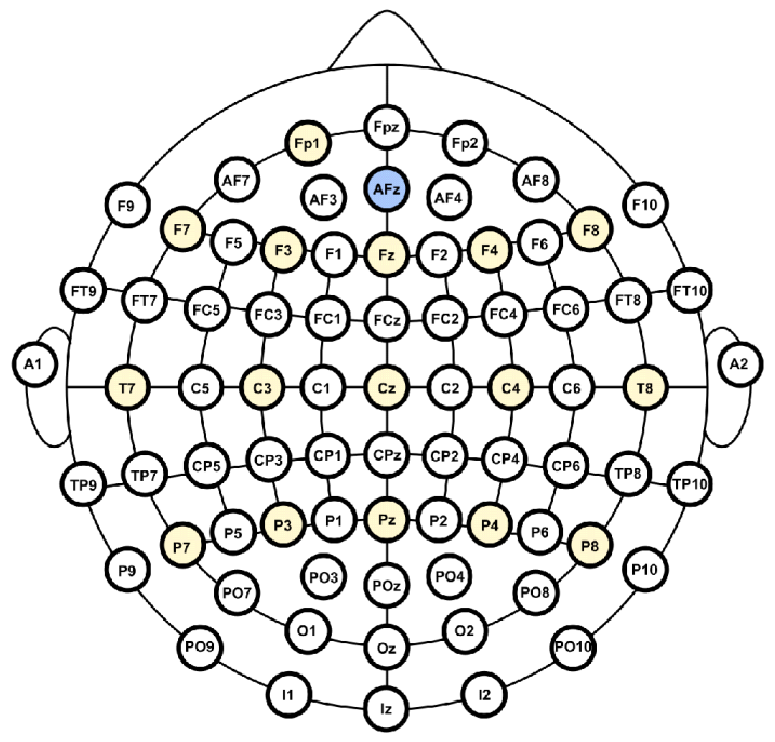
\includegraphics[width=0.4\linewidth]{./img_dev/10-10_sketch}
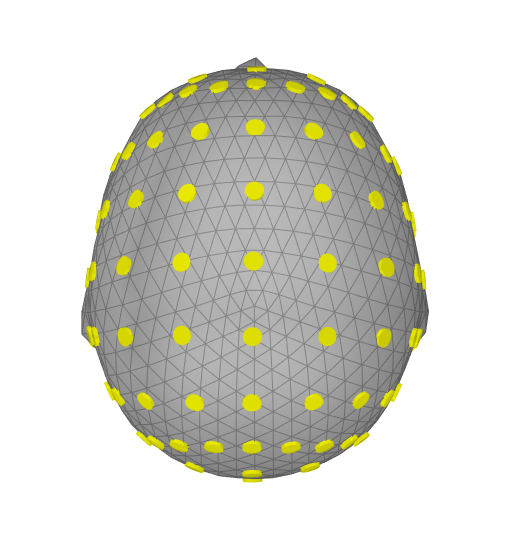
\includegraphics[width=0.25\linewidth]{./img_dev/EEG_3D_Subject_ICBM152_2019b_top}
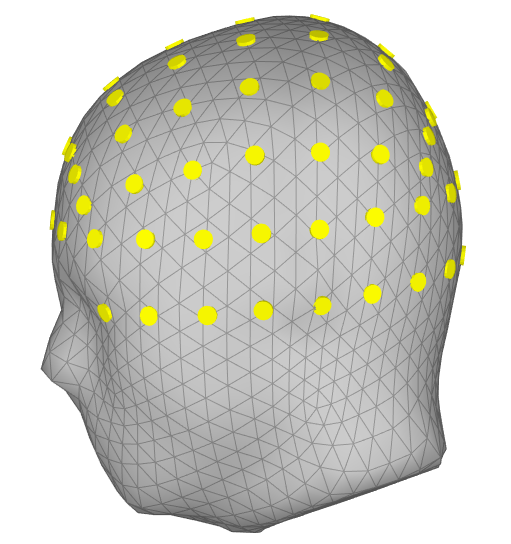
\includegraphics[width=0.25\linewidth]{./img_dev/EEG_3D_Subject_ICBM152_2019b_left}
%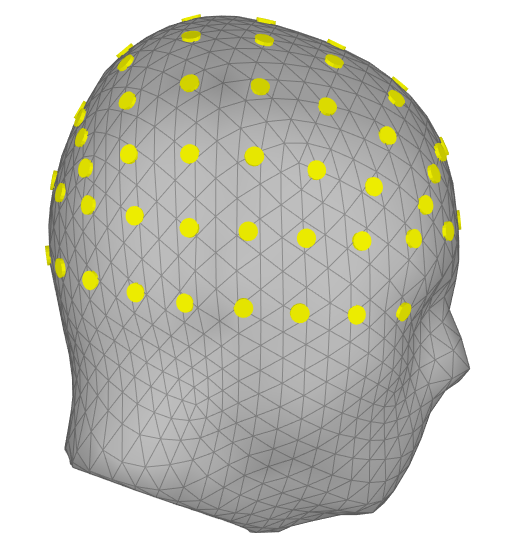
\includegraphics[width=0.25\linewidth]{./img_dev/EEG_3D_Subject_ICBM152_2019b_right}
\caption{Electrode Placement according to the 10-10 International System.}
\label{fig:1010system}
\end{figure}

%\subsubsection{Synthetic data protocol}

Following the forward model from equation \eqref{eq:general}, the synthetic data is constructed by (1) constructing $\SA$ based on a source distribution described later, then (2) constructing $\nu$ and $\varepsilon$ to meet a prescribed Signal-to-Noise Ratio (SNR), and finally (3) constructing $\Y$ as in the forward model.

The source distribution, $\SA$, is constructed by considering a small source patch.
%
The dipoles in the source patch are selected as those being close to a seed dipole, indexed by $n^*$, which is selected randomly.

After selecting the seed dipole, indexed by $n^*$, $\SA$ is constructed as
\begin{equation}
\SA(n) = f\ppar{ \nnorm{\rr_n-\rr_{n^*}} / \kappa }
\end{equation}
with $\rr_n$ the location of the $n$-t dipole, $f:\R_+\rightarrow \R_+$ a decreasing function and $\kappa>0$ a scaling parameters.
%
See figure \ref{fig:exaple_true} for a representation of the location and extent of the extended source.

\begin{figure}
\centering
%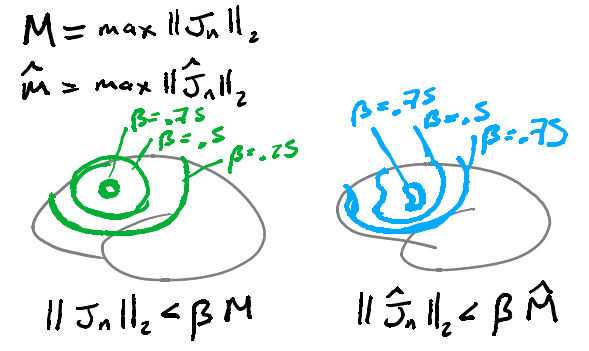
\includegraphics[width=0.8\linewidth]{./img_dev/nsCurves1}
%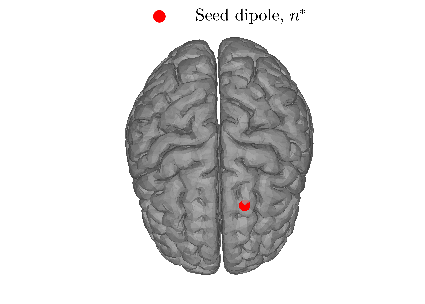
\includegraphics{./img/gauss_center}
%\includegraphics{./img/square_GroundTruth}
\includegraphics{./img_MATLAB/square_GroundTruth}
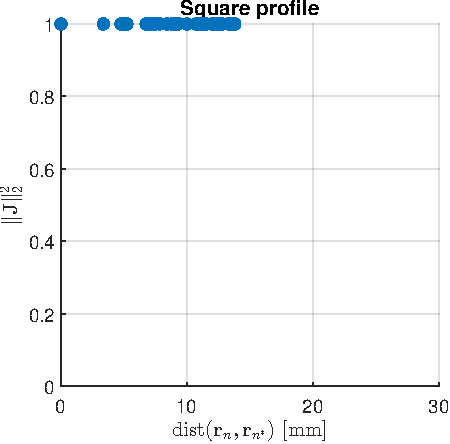
\includegraphics[height=2in]{./img_MATLAB/square_Profile}
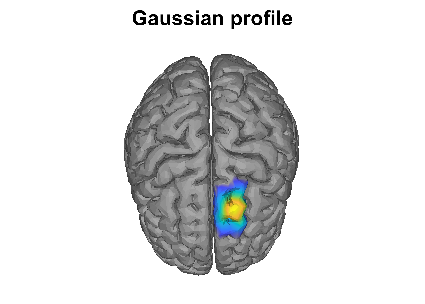
\includegraphics{./img_MATLAB/gauss_GroundTruth}
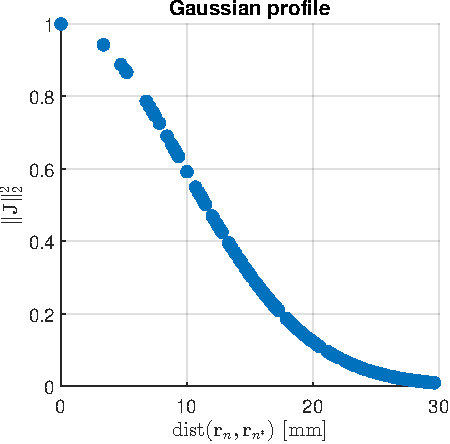
\includegraphics[height=2in]{./img_MATLAB/gauss_Profile}
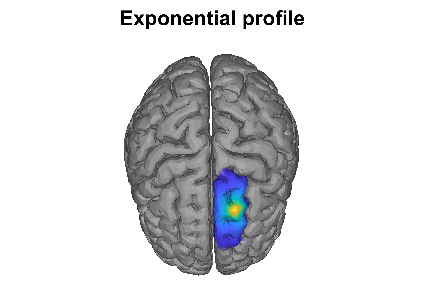
\includegraphics{./img_MATLAB/exp_GroundTruth}
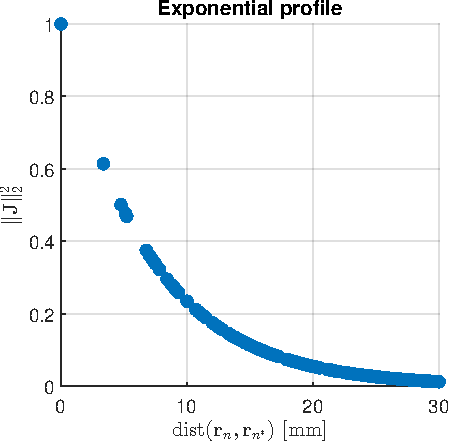
\includegraphics[height=2in]{./img_MATLAB/exp_Profile}
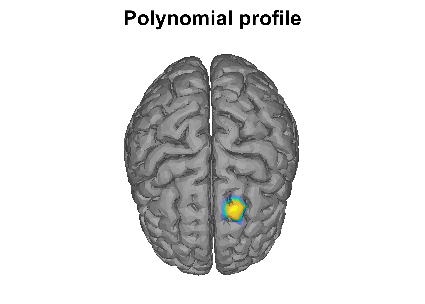
\includegraphics{./img_MATLAB/circ_GroundTruth}
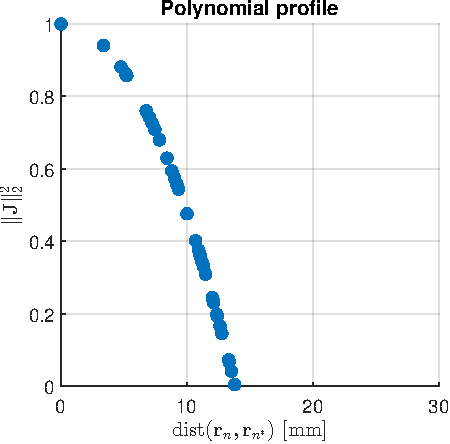
\includegraphics[height=2in]{./img_MATLAB/circ_Profile}
\caption{Cortical patch used for the creation of synthetic data.}
\label{fig:exaple_true}
\end{figure}

%This type of configuration is referred to as `source patches' or `extended sources' since it occupies an area too large to be modeled as a single dipole.

For the synthetic data in this section, the dipole $n^*$ was selected within the frontal cortex for visibility.
%
We use the square profile, defined by using
\begin{equation}
f(x) = \begin{cases}
1, &\text{if } x\leq 1 \\
0, &\text{otherwise}.
\end{cases}
\end{equation}
and $\kappa = $ 12.6 \si{mm}, to obtain a source patch with an area of approximately 5 \si{cm^2}.

For simplicity within the model formulation, we considered no internal noise ($\nu=0$) and independent Gaussian noise at the sensors, i.e. $\varepsilon_m \sim\norm\ppar{0, \sigma_m^2}$ for $m = 1, \dots, M$ for some parameters $\sigma_m\geq 0$.
%
Under these conditions, the distribution of $\Y$ is given by
\begin{equation}
\ppar{\Y \given \SA} =
\norm\ppar{ \G\, \SA, \diag{\sigma_1, \dots, \sigma_M}^2 }
\end{equation}

The channel SNR (in dB) for the $m$-th sensor is given by
\begin{equation}
\text{SNR}_m = 
10\, \log_{10}\ppar{ \frac{ \ppar{ \spar{\G\, \SA}(m)}^2 }{\sigma_m^2} }
\end{equation}
With a prescribed SNR value, the parameters $\sigma_m$ are selected as follows
\begin{equation}
\sigma_m^2 = 
10^{{-{SNR}/{10}} }
\spar{\G\, \SA}(m)
\end{equation}

For the synthetic data in this section, we consider an SNR level of 20 dB, which we consider a low-noise condition.


%%%%%%%%%%%%%%%%%%%%%%%%%%%%%%%%%%%%%%%%%%%%%%%%%%%%%%%%
%%%%%%%%%%%%%%%%%%%%%%%%%%%%%%%%%%%%%%%%%%%%%%%%%%%%%%%%

%\section{Multi-modal asymmetric methods}
%
%A common framework
%to enhance ESI is to incorporate 
%`information' from the additional {modalities} of data:
%%and then constrain ESI to it.
%%
%%Multiple authors have explored the idea 
%%of enhancing 
%%the EEG Source Localization
%%by adding data from other `modes' of data: 
%MEG, MRI/fMRI\cite{he2008multimodal, huster2012methods}, PET, fNIRS\cite{fnirs}, etc.
%(Figure based on \cite{he2008multimodal}).
%%of using additional data to aid the EEG Source Localization, would it be MEG.
%\begin{figure}
%\centering
%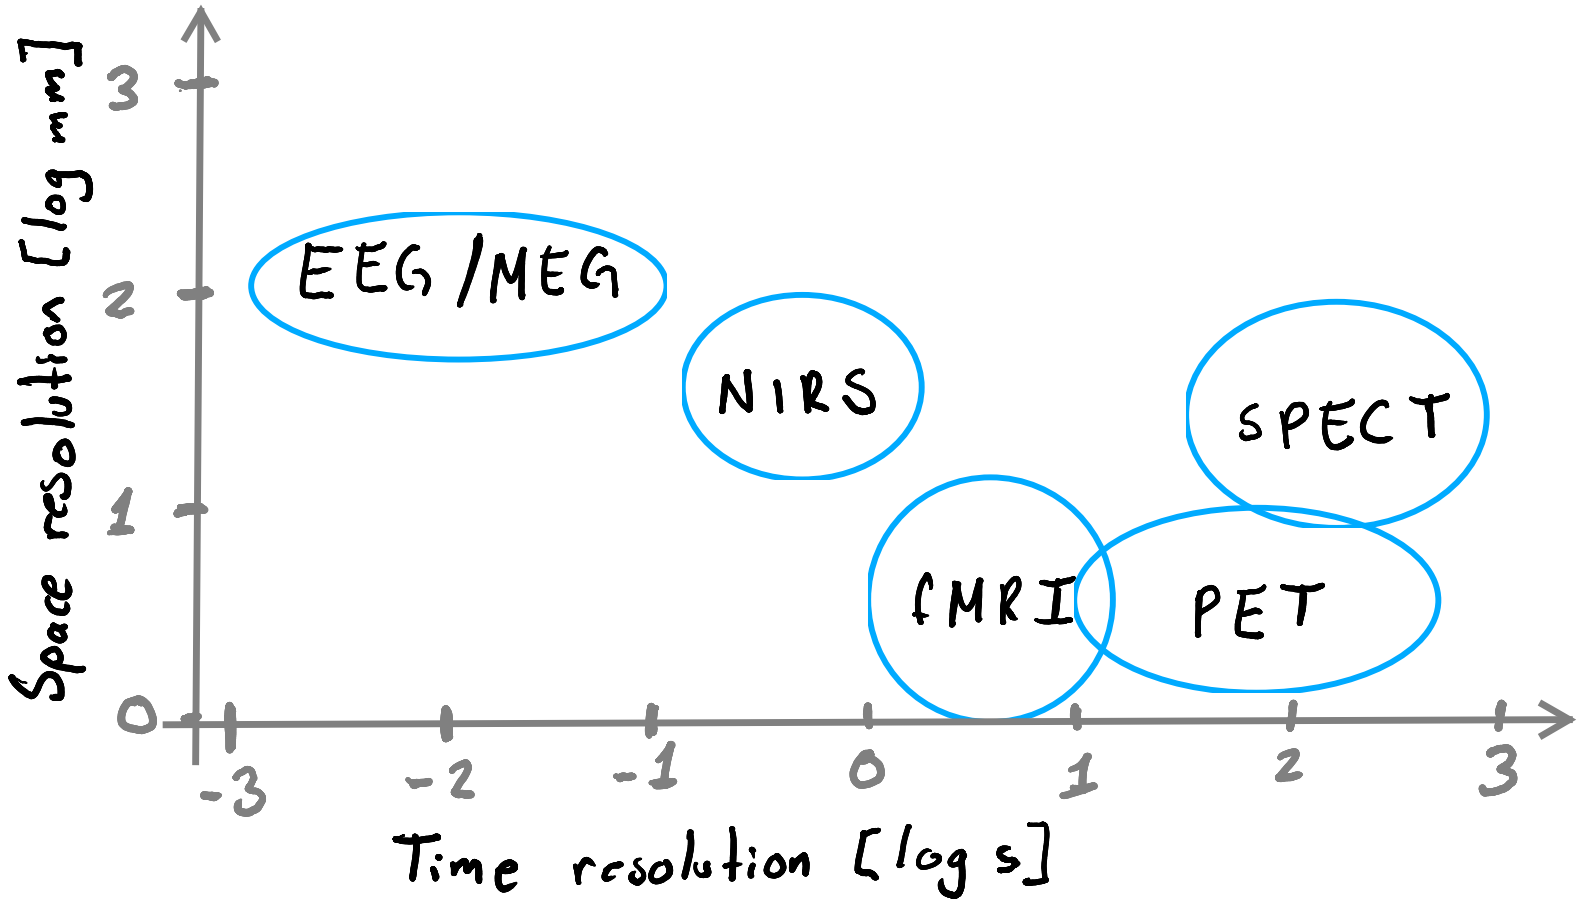
\includegraphics[width=0.65\linewidth]{./img_final/sketch07}
%\caption{PET=Positron Emission Tomography, NIRS=Near Infrared Spectroscopy, SPECT=Single-Photon Emission Computed Tomography}
%\end{figure}
%
%
%One big conceptual challenge for multimodal data integration is to model the interaction of the underlying physical phenomena. 
%%
%Focusing only on unilateral interactions results in asymmetric data integration.
%
%%For
%%asymmetric data integration, 
%%such as enhanced ESI, 
%%some bilateral interactions may be simplified. 
%%Thus 
%
%{Asymmetric data fusion} is the extraction of some parameters from one modality, which then are used to further the  for ESIanalysis of the other modaliFor ESI, the obtained parameters are typically used within the penalty functions.
%%Some simplifying assumptions considered in the literature for asymmetric data fusion for ESI are:
%%A common framework
%%Some techniques used in the literature 
%%to ESI enhancing is to extract `information' from the additional modalities and then constrain ESI to it.
%Some of the parameters extracted include:
%\begin{itemize}
%    \item Correlation networks
%    \item Statistical Parametric Maps (SPM)
%    \item Hidden activation variables \cite{fire}
%\end{itemize}

